\chapter{Technické základy}

V této kapitole čtenáře seznámíme s herním enginem Unity \cite{Unity} do míry potřebné k pochopení zbytku práce. Stručně nastíníme architekturu, kterou pro tvorbu herních systémů tento engine podporuje, a zmíníme některé jeho vestavěné knihovny - především se podrobně zaměříme na integrovaný fyzikální subsystém.


\section{Herní engine Unity} \label{unityEngineIntroSection}

První verze enginu Unity byla představena v roce 2005. Od té doby bylo vydáno mnoho verzí, přidáno mnoho funkcionalit a mnoho dalších prohlášeno za zastaralé. Tvůrcům se dařilo držet krok s dobou, v dnešní době jde o velmi vyspělý a moderní engine, který uživatelům nabízí \textbf{široký ekosystém nástrojů}, ať už jde o integrované komponenty, nebo balíčky třetích stran. 

Jednou z jeho velkých sil je \textbf{všestrannost} - zvládá stejně dobře 2D i 3D hry, výsledný spustitelný produkt lze vyexportovat pro širokou škálu platforem - desktopové, mobilní, konzole i web.

Pro programování herní logiky je zde podporován jazyk C\#. Jako runtime je dosud používáno postarší \textbf{Mono}, které umožňuje nanejvýše \textbf{C\# verze 9} s pár drobnostmi nepodporovanými, avšak stále jde o vcelku moderní jazyk, který programátorovi umožňuje pohodlnou práci. Interakce s knihovnami třetích stran, které závisejí na některých součástech moderního frameworku .NET, může činit problémy, avšak typicky nejde o nepřekonatelnou překážku.

Jde o \textbf{komerční produkt s uzavřenou licencí}, avšak cenová politika je více než přívětivá. Pro nekomerční projekty a projekty nepřesahující určitou hranici celkového ročního zisku je \textbf{použití enginu zcela zdarma}. Právní úprava nijak nebrání vydávání samostatných projektů v enginu tvořených pod opensource licencí. Dokumentace není celkově na špatné úrovni a těch pár míst, kde pokulhává, vynahrazují velmi živá komunitní fóra.
\bigbreak
V této kapitole si představíme základní principy použití enginu v rozsahu nutném pro vysvětlení zbytku práce. Jejich kompletnější popis čtenář najde v oficielní dokumentaci \cite{Unity}. 

\subsection{Herní objekty a komponenty}

\subsubsection*{Scéna}
Základním prvkem je \textbf{scéna} - ta odpovídá jedné oblasti ve hře. Scéna může být aktivní vždy jen jedna, hráč mezi nimi přechází.

\subsubsection*{Herní objekt}
Scéna je popsána hierarchií \textbf{herních objektů} (třída UnityEngine.GameObject). Každý herní objekt je definován svou pozicí v hierarchii (svým otcem), transformační maticí (udává pozici v herním světě) a jménem\footnote{Jméno slouží pro dokumentační a debugovací účely.} a najdeme v něm (volitelně prázdný) list dodatečných komponent.

\subsubsection*{Komponenty}
Komponenty jsou základními modulárními stavebními prvky, ze kterých skládáme herní logiku. Herní engine nám poskytuje velké množství již hotových - např. jednu, skrze kterou lze definovat grafickou reprezentaci objektu, další, jež nese zodpovědnost za vykreslení této reprezentace - takto by bylo možné pokračovat velmi dlouho. Uživatel může vytvořit vlastní typ komponenty tak, že ve skriptu definuje třídu dědící z UnityEngine.MonoBehavior. Následně mu již nic nebrání vybrat si v editoru herní objekt a novou instanci komponenty (její jméno odpovídá jménu třídy) do něj přidat.

Každá komponenta může nést data a herní logiku, ty jsou definovány jednoduše skrze instanční proměnné a metody.  

\subsubsection*{Transform}

Speciální komponentou je UnityEngine.Transform. Tu nalezneme na každém herním objektu, reprezentuje jeho \textbf{transformační matici} a \textbf{pozici v objektové hierarchii}. Každý objekt má vlastní matici, která definuje jeho polohu, rotaci a škálování - lokálně vůči otci. Celková transformace objektu je určena vynásobením této matice se součinem matic všech předků.

\subsubsection*{Serializace} \label{gameObjectSerializationSubSubSection}

Při práci na hře často narazíme na situaci, kdy by bylo užitečné moci nastavit část dat, které komponenta nese, ručně z editoru. Engine nám toto umožní.

Jakoukoliv proměnnou, která je deklarovaná jako public či anotovaná atributem [UnityEngine.SerializeField], se editor pokusí poskytnout k editaci.
\begin{itemize}
    \item Primitivní a vestavěné typy zpravidla nečiní problém.
    \item Pro typy dědící z UnityEngine.Object je poskytnuto pole, do kterého je možné přetáhnout jakýkoliv objekt ze scény či prefab.
    \item Uživatelsky definované třídy musí být anotovány jako [System.Serializable] - jejich editor pak sestává rekurzivně z políček odpovídajících jejich proměnným, instance je vytvořena automaticky skrze výchozí konstruktor.
    \item Proměnná nesmí být typu rozhranní, až do nedávna nebyly podporovány ani typy s generickým parametrem.
    \item Z datových struktur jsou podporovány pouze obyčejné pole a System.Collections.Generic.List<>.
\end{itemize}
Dalším omezením je, že musí jít vždy o proměnné - properties podporovány nejsou.

Tato omezení - především nemožnost používat interfacy a properties\footnote{Nepodporu složitějších datových struktur lze kompenzovat použitím pokročilých technik pro vytváření vlastních editorových oken. Nepodpora generik pak činí problém spíše jen u sealed typů a structů, ze kterých není možné odvodit negenerického potomka.} - mohou programátorovi značně ztížit snahy o dodržování dobrých praktik objektového programování\footnote{Důsledkem této limitace je, že napříč naší codebase čtenář narazí na mnoho typů, které používají standardní jmennou konvenci ITypeName - s cílem komunikovat záměr, že myšlenkově plní roli rozhraní - avšak jsou implementovány jako abstraktní třída (mnohdy odvozená z UnityEngine.MonoBehavior).}.

Důvodem je, že tato úprava polí v editoru je specielním případem použití \textbf{standardního serializačního subsystému} enginu Unity. Na ten narazíme kdekoliv, kde je třeba interně ukládat herní stav do podoby, ze které bude možné jej později rekonstruovat. Mimo jiné je rovněž zodpovědný za to, aby ve finální sestavené verzi hry bylo načítání scény pro hráče co nejrychlejší. Je tedy jen přirozené, že je koncipován především pro co možná nejvyšší výkon - z čehož plynou výše zmíněná omezení.

\subsubsection*{Prefaby}
Standardní serializační systém však programátorovi přináší i mnoho výhod. Jeho nápomocí nám je umožněno jednoduše přetáhnout herní objekt z objektové hierarchie do souborového systému a vytvořit z něj tzv. \textbf{prefab}. Takto osamostatněný objekt můžeme následně referovat libovolněkrát v libovolné scéně a systém se postará, aby veškeré změny, které byly provedeny přímo na prefabu, byly přeneseny do jednotlivých instancí, zatímco změny oproti prefabu, kterých jsme se dopustili na konkrétní instanci, zůstanou zachovány. Rovněž je možné vytvořit \textbf{variantu prefabu} - samostatný prefab, který se odkazuje na jiný prefab jakožto svou předlohu a vůči ní přibaluje nějaké změny. 

Jak vidíme, jde o mocný nástroj umožňující organizaci herních objektů podobně flexibilním způsobem, jaký nabízí dědičnost v oblasti objektového programování. 

\subsubsection*{Komunikace mezi komponentami} \label{communicationBetweenComponentsSubsubsection}

Jakákoliv trochu komplexnější herní logika se neobejde bez vzájemné komunikace mezi komponentami. Unity nám k tomuto účelu nabízí hned několik základních cest.

První z nich je zkrátka na instanci druhé komponenty \textbf{zavolat metodu, kterou chceme}. Výhodou je, že metoda může mít libovolné množství argumentů, být generická, ... celkově je možné využívat plně možností, které jazyk C\# poskytuje. Nevýhodou je, že musíme mít přímý odkaz na instanci, na které volání uskutečňujeme.

Druhou možností je \textbf{UnityEvent}. Jde o obdobu klasických C\# delegátů, která však podporuje serializaci a je ji tedy možné konfigurovat z editoru. S její pomocí komponenta může definovat callbacky, do kterých je následně v editoru zaregistrováno libovolné množství posluchačských metod patřících ostatním komponentám. Zavoláním metody Invoke() na instanci UnityEvent jsou následně zavolány všechny posluchačské metody, jedna po druhé.

Poslední možností je \textbf{posílání zpráv}. Tento mechanismus je hojně používán pro komunikaci mezi komponentami a systémem. Princip je jednodchý: na libovolném herním objektu je možné zavolat metodu SendMessage() - jejím parametrem je jméno metody, volitelně ještě libovolný objekt jako argument. Systém projde všechny komponenty náležící danému objektu a pokud nějaký z nich definuje (jedno zda veřejnou či privátní) metodu, jejíž hlavička odpovídá jménu a typu argumentu, jež jsme metodě SendMessage předali, všechny takovéto metody budou jedna po druhé zavolány.

\subsubsection*{Jak hledat komponenty} \label{howToSearchForComponentsSubsubsection}

V mnoha případech potřebujeme s instancí jiné komponenty komunikovat přímo. Jakým způsobem lze tedy odkaz na ni získat?

Nejjednodušší možností je na naší komponentě zavést serializovatelnou proměnnou, do které odkaz na druhou komponentu doplníme v editoru. 

Pokud tato možnost nepřipadá v úvahu, či je komponent mnoho a přetahovat všechny by bylo přespříliš úmorné, Unity nabízí mnoho cest, jak scénu prohledávat. Mezi základní patří:

\begin{itemize}
    \item \textbf{gameObject.GetComponent<TComponent>()} - Voláme na konkrétní instanci herního objektu. Vrátí první komponentu typu TComponent, jež se v objektu nachází, popř. null. TComponent může být konkrétní typ komponenty, rovněž to však může být rozhraní. Existuje také varianta GetComponent\underline{s}<TComponent>(), která iteruje všechny takové komponenty, pokud jich je více. Také GetComponent(s)InParent() a GetComponent(s)InChildren(), které prohledávají celou objektovou hierarchii směrem od objektu nahoru/dolu.
    \item \textbf{UnityEngine.Object.FindFirstObjectByType<TObject>()} - Statická metoda. Podobné chování jako GetComponent, avšak prohledává celou aktivní scénu. 
    \item \textbf{UnityEngine.GameObject.FindByTag()} - Rovněž prohledává celou scénu. Pro každý herní objekt je možné v editoru nastavit specielní poznávací symbol - tag - podle něj zde vyhledáváme. Vrací odkaz na herní objekt, na něm typicky ještě bude nutné zavolat GetComponent. Toto je obecně doporučovaný způsob, jak získávat odkaz na singletony.
\end{itemize}

Je však třeba podotknout, že všechny tyto možnosti zpravidla vykonávají nějakou formu lineárního hledání a nejsou tedy zcela efektivní. Velmi doporučované je provádět hledání pokud možno jen jednou při aktivaci naší komponenty, a jeho výsledek si "nakešovat" do proměnné.

\subsection{Herní smyčka}

Typická videohra běží v \textbf{nekonečné smyčce}. Jsou načteny vstupy, provedena aktualizace herního stavu, následně vykreslena grafika - jakmile je hotovo, opakujeme. 

V Unity je herní smyčka plně v režii systému, programátor může ve svých skriptech pouze \textbf{poslouchat na události}, které v jejím průběhu nastanou. Ty jsou mu typicky komunikovány pomocí výše popsaného systému posílání zpráv (viz \ref{communicationBetweenComponentsSubsubsection}).
Typickými takovými zprávami jsou:

\begin{itemize}
    \item \textbf{Update()} - Volána jednou za každý snímek. Zde by měla být updatována herní logika. Čas uplynulý od minulého snímku není předáván jako argument, nýbrž ho lze vyčíst ze statické proměnné UnityEngine.Time.deltaTime.
    \item \textbf{Start()} - Volána jednou za život objektu, těsně před tím, než je zavolán jeho první Update(). Zde by typicky mělo probíhat hledání dalších komponent a podobné inicializační operace.
    \item \textbf{Awake()} - Volána okamžitě po vytvoření objektu, tedy dříve než Start. Některé další zprávy mají okrajové případy, ve kterých rovněž mohou být zavolány dříve než Start - pokud to hrozí, je třeba provést inicializaci zde.
    \item \textbf{OnDestroy()} - Volána při zničení komponenty. Zde může uvolnit držené zdroje.
\end{itemize}
Zajímavou vlastností je, že komponenta může být nastavena jako \textbf{neaktivní} - v takovém případě nedostává zprávy Update a volání Start je odloženo. Awake a OnDestroy však stále volány jsou.

Rovněž je užitečné vědět, že veškeré zprávy herní smyčky jsou volány \textbf{sekvenčně na hlavním vlákně}. Multithreading v Unity nalezneme pouze na specifických místech, a na těch si tvůrci dali záležet, aby byl uživatel velmi důrazně varován.


\subsection{Vstup} \label{unityInputExplanationSubsection}

Pro čtení uživatelského vstupu Unity nabízí několik možností - zde si představíme tu nejjednodušší, kterou je statická třída \textbf{UnityEngine.Input}.

Jde o velmi starou část enginu, která je vázána potřebou zpětné kompatibility do některých ne-zcela-ideálních rozhodnutí, avšak pro svou jednoduchost na základní použití v porovnání s alternativami je stále velmi oblíbená. 

Základními službami, které poskytuje, jsou:
\begin{itemize}
    \item \textbf{UnityEngine.Input.GetKey()} - Této funkci předáme jako argument klávesu (jeden z prvků enumu - zahrnuje specielní klávesy jako Esc nebo Shift) a z návratové hodnoty zjistíme, zda klávesa je či není aktuálně stisknutá. Rovněž nalezneme varianty GetKeyDown/GetKeyUp, které vrací true pouze ve snímku, kdy stisk začal/skončil.
    \item \textbf{UnityEngine.Input.GetAxis()} - V nastavení projektu je možné konfigurovat pojmenované "osy vstupu", které mohou odpovídat pohybu myši, joysticku nebo dvojici kláves. Tato funkce nám pro osu daného jména vrátí příslušnou hodnotu v intervalu [-1; 1] (jak silně doleva/doprava).
    \item \textbf{UnityEngine.Input.mousePosition} - Souřadnice pixelu obrazovky, kde se nalézá kurzor myši. Máme-li k dispozici kameru, která odpovídá obrazovce (typicky UnityEngine.Camera.main), takto získáme paprsek v herním světě: camera.ScreenPointToRay(UnityEngine.Input.mousePosition).  
\end{itemize}

Aktualizace vstupu probíhá každý snímek těsně před voláním funkcí Update() - ta je tedy pro herní logiku, jež ze vstupu čte, ideálním místem. Při čtení vstupu např. uvnitř FixedUpdate() se může stát, že některé krátce trvající události (především KeyDown, KeyUp) nebudou zaznamenány.

\subsection{Knihovny}

Kromě standardní knihovny jazyka C\# poskytuje Unity \textbf{mnoho dalších knihoven} nabízejících funkcionalitu užitečnou specificky při tvorbě videoher.

Samozřejmě zde najdeme mnoho nástrojů pro pokročilou \textbf{interakci s hierarchií herních objektů} - ničit objekty či vytvářet nové za běhu není problém. 

Dále zde najdeme například široký výběr \textbf{matematických primitiv} - vektory (2D a 3D) a matice umožňující provádět základní operace známé z lineární algebry a mnoho typů reprezentujících další geometrické objekty jako přímky či roviny.

Velkými tématy pro videohry jsou jak známo například \textbf{vykreslování grafiky} s pomocí GPU, \textbf{animace}, či \textbf{navigace herních postav terénem}. Pro každou z těchto oblastí a mnoho dalších disponuje Unity dedikovaným subsystémem. O šířce jeho záběru se lze přesvědčit v oficielní dokumentaci \cite{Unity}.

\section{Fyzikální subsystém enginu Unity}

Jedním z těchto subsystémů, který budeme napříč naší prací extenzivně využívat, je ten pro fyzikální simulaci. Jeho náplní práce je vypočítávat pohyby a síly působící mezi objekty herní scény, způsobem velmi podobným tomu, jaký známe z klasické středoškolské kinematiky a dynamiky pevného tělesa. Unity poskytuje takové systémy dokonce dva\footnote{Více když neopomeneme Unity DOTS.} - jeden operující v 3D prostoru, druhý pro 2D. Oba jsou samostatnými celky a nesdílejí žádné společné součásti. Ve zbytku práce budeme fyzikálním subsystémem automaticky myslet ten pro 3D.   

Užitečnou informací je, že tento subsystém je pouze tenkým rozhraním pro podmnožinu funkcionality backendu, kterým je Nvidia PhysX \cite{PhysX}. Dokumentaci Nvidie \cite{PhysX} lze tedy doporučit k pročtení komukoliv, kdo chce získat hlubší porozumění celkovému fungování systému, než jaké nabízí oficielní dokumentace Unity.

\subsection{Základy}

Pro zaručení větší stability je pravidlem, že by fyzikální simulace měla být aktualizována ve fixních časových intervalech. Unity tedy pro tyto účely nabízí \textbf{fixní herní smyčku}, která běží (rovněž v hlavním vlákně) paralelně s tou klasickou. Ve skriptu můžeme poslouchat na zprávu FixedUpdate() - ta je zavolána každý fixní snímek, těsně před vykonáním kroku fyzikální simulace. 

Subsystém si vede vlastní interní reprezentaci celé scény. Nad tou vykonává veškeré výpočty, až po dokončení celého kroku simulace podle ní updatuje transformy objektů ve scéně. 

\subsection{Rigidbody}

Základní komponentou je Rigidbody. Jeho přidáním získá herní objekt schopnost být ovlivňován silami a působit silami na ostatní objekty.

Přímo na této komponentě můžeme nastavit jeho základní parametry jako je váha, poloha těžiště, zda na něj má působit gravitace či zda je \textbf{kinematické}.

\textbf{Nekinematické} rigidbody má pohyb plně ovládaný fyzikální simulací. Každý fyzikální snímek je systémem pohnuto dle své aktuální rychlosti (rigidbody.velocity), tu mohou ovlivňovat síly, které na něj působí - vyvolané buď gravitací, kolizemi, nebo aplikací ze skriptu (rigidbody.AddForce(), rigidbody.AddTorque()).

\textbf{Kinematické} oproti tomu může působit (kolizními) silami na ostatní objekty, avšak samo fyzikálním systémem ovládané není - jeho pohyb je plně v režii programátora, který ho může vykonávat klasicky updatováním komponenty Transform.

Mezi těmito dvěma stavy \textbf{lze přepínat} jednoduše úpravou flagu (rigidbody.isKinematic). Nečiní tedy problém mít např. meč, který je plně fyzikálně simulovaný, ale při sesílání kouzla se přepne a přehraje předpřipravenou animaci, či naopak postavu, která je ovládána animacemi, ale v okamžiku smrti se změní ve fyzikálně simulovanou ragdoll.

\subsection{Collider} \label{collidersPhysicsIntroSubsection}

Collidery jsou komponenty, které určují pro účely fyzikálního systému tvar objektu a umožňují mu kolidovat s ostatními objekty. 

V komplikovanější scéně jich často v jednom okamžiku najdeme vyšší stovky až tisíce. Proto je jedním z nejdůležitějších úkolů každého fyzikálního systému zaručit, aby detekce kolizí probíhala \textbf{co nejefektivněji} a byl tím pádem umožněn běh hry v reálném čase.

Jedním z prostředků, které pomáhají toho dosáhnout, je použití \textbf{primitivních tvarů} namísto colliderů přesně odpovídajících grafickému meshi objektu\footnote{Collidery definované meshem do jisté míry podporovány jsou, ale nesou mnohá omezení. Jejich použití má smysl převážně pro statický terén herního světa a zde se jimi nebudeme zaobírat.}. Unity nám nabízí tři - \textbf{krychli, kouli a kapsli}\footnote{válec s polokoulemi na obou koncích} - na objekt je umístíme přidáním odpovídající komponenty (BoxCollider, SphereCollider, CapsuleCollider). Komplexnějších tvarů dosahujeme skládáním více colliderů dohromady\footnote{Skutečně jde o jedinou možnost. Bystrý čtenář by mohl očekávat, že šikovným použitím transformační matice na herním objektu, kde se collider nalézá, by neměl být problém např. z BoxCollideru vytvořit rovnoběžnostěn. V dokumentaci se však lze dočíst, že podobné transformace ústí v nedefinované chování.}. Tím lze samozřejmě vytvořit pouze hrubou aproximaci skutečného tvaru objektu, v praxi se to však ukazuje jako naprosto dostatečné - při umném rozmístění hráčský zážitek obvykle nijak netrpí.

\textbf{Tvar rigidbody} stanovíme tak, že umístíme libovolné množství colliderů do objektu, kde je komponenta rigidbody definována, či libovolně do jeho potomků. Všechny tyto collidery jsou následně považovány dohromady za jeden kompozit, který popisuje celkový tvar rigidbody. 

\textbf{Statickým} colliderem nazveme takový, který není součástí hierarchie žádného rigidbody. Takový collider je schopen kolidovat s rigidbodies a sloužit pro ně jako překážka. Je považován za pevnou součást scény a jeho transform by měl po celé trvání hry zůstat stejný (pohyb může ústit v nedefinované chování). Chceme-li collider s chováním statického, kterým však můžeme bez obav pohybovat, umístíme jej do kinematického rigidbody. Statické a kinematické collidery přirozeně vzájemně nekolidují.

Jemnější kontrolu nad tím, \textbf{co s čím může kolidovat}, nám poskytují tzv. \textbf{Layers}. Jde o pojmenované skupiny, kterých může být definováno nanejvýš 32 a nastavují se jako vlastnost herního objektu (gameObject.layer). V globálním nastavení herního projektu lze následně pro konkrétní páry vrstev kolize zakázat - takové dva objekty následně projdou bez reakce skrze sebe, kolize nebude ani detekována. Pro jemnější kontrolu je každý collider vybaven whitelistem a blacklistem vrstev, pomocí kterého lze globální nastavení přepsat. Ještě jemnější kontroly pak je možné dosáhnout ze skriptu - pomocí statické metody UnityEngine.Physics.IgnoreCollision() lze zakázat kolize pro konkrétní pár colliderů\footnote{Takto je však možné pouze kolize selektivně zakázat, nikoliv povolit. IgnoreCollision(a, b, false) pro a, b na vrstvách, které se ignorují, stále zanechá tento pár neschopný kolize.}.

Často potřebujeme pouze detekovat, že ke kolizi dvou objektů došlo, aniž bychom z toho vyvozovali nějaké fyzikální implikace - např. pokud fotbalový míč vstoupí do vnitřní části branky, chceme započítat gól, avšak rozhodně nechceme, aby vnitřek branky sám míči jakkoliv bránil ve vstupu. Pro tyto účely slouží flag \textbf{collider.isTrigger}. Po jeho zaškrtnutí collider přestane na kolidující objekty působit silami bránícími v průniku, stále však budou kolize detekovány.

Každá probíhající kolize je kolidujícímu hernímu objektu komunikována \textbf{posíláním zpráv} OnCollisionEnter, OnCollisionStay a OnCollisionExit. V případě trigger collideru jsou posílány obdobné zprávy začínající na OnTrigger - rozdíl mezi nimi je ten, že argument OnCollision obsahuje podrobné informace o bodech dotyku a silách použitých k rozřešení, OnTrigger poskytne pouze druhý collider. 

Velmi důležitým aspektem tohoto chování, který oficielní dokumentace zcela zamlčuje, je, že v případě Rigidbody jsou OnCollision zprávy poslány pouze do kořenového herního objektu - i v případě, že konkrétní kolidující collider se nachází v jednom z jeho potomků. OnTrigger zprávy jsou pak poslány vždy jak do kořenu, tak do konkrétního triggerovaného objektu. Do žádného z dalších objektů v hierarchii však stále ne. Toto má velký význam v kontextu toho, že ani OnCollision, ani OnTrigger svým argumentem neposkytují odkaz na konkrétní collider, jehož prostřednictví naše rigidbody zkolidovalo (pouze na ten, který zkolidoval s námi) - dozvědět se spolehlivě\footnote{Nespolehlivou cestou je např. collision.GetContact(0).thisCollider. Dle dokumentace máme mít zaručeno, že collision vždy bude obsahovat alespoň jeden kontakt. To však platí s výjimkou OnCollisionExit a ve skutečnosti se tak často neděje ani v ostatních zprávách.}, který to byl, je tedy, především pro zprávu OnCollision, velmi netriviální problém, který může mít dalekosáhlé následky pro některé aspekty architektury našeho systému.

Poslední důležitou problematikou, kterou letmo zmíníme, jsou metody \textbf{detekce kolizí}. Výchozí je detekce diskrétní - ta zkrátka každý krok simulace projde celou scénu a provede testy, zda aktuálně nějaké objekty mají neprázdný průnik. To je rychlé a v mnoha případech funguje dostatečně dobře. Problém však činí rychle letící či malé objekty - klasickým případem je projektil vystřelený z palné zbraně. U toho se může stát, že v jednom snímku je na jedné straně stěny, ve snímku následujícím již zcela na straně druhé, aniž by jakákoliv kolize byla detekována - projektil tzv. \textbf{protuneloval}. Řešení tohoto problému nabízí \textbf{spojitá detekce kolizí} - ta propočítává celkovou dráhu objektu v průběhu času mezi snímky a ústí tedy v horší výkon. Konkrétní implementace, které Unity nabízí, budou velmi relevantní pro \ref{swordCollisionsSection} a podrobně je tedy představíme tam.

\begin{figure}[ht]\centering
    \center
    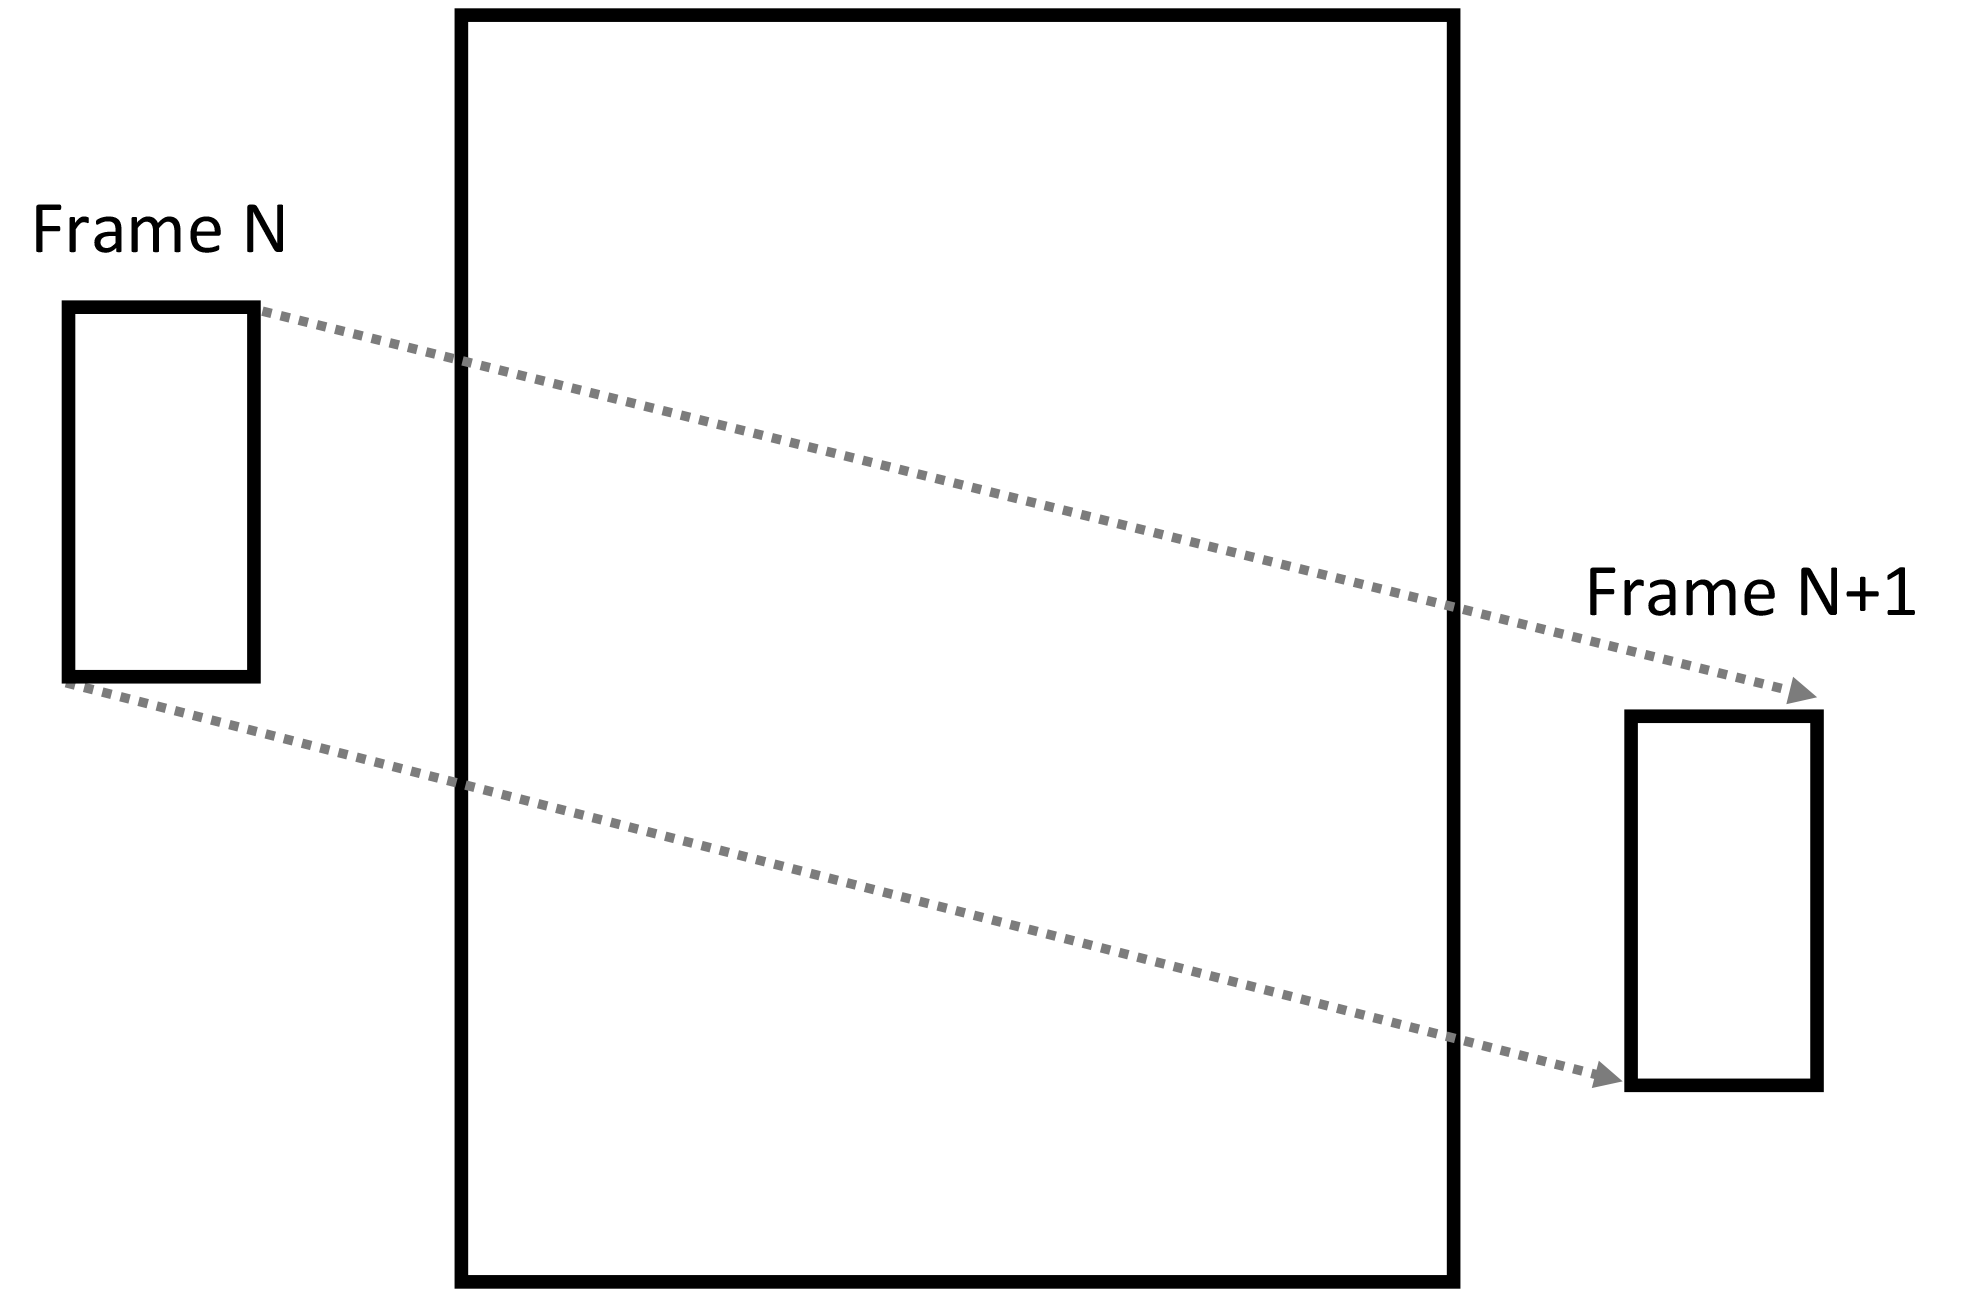
\includegraphics[width=90mm]{../img/diagram-tunneling.png}
    \caption{Diagram zachycující protunelování malého objektu skrze překážku}
    \label{obr03:tunneling}
\end{figure} 

\subsection{Joint}

Jointy jsou nástrojem, který umožňuje definovat \textbf{složitější vztahy mezi několika rigidbodies}. Najdeme zde například FixedJoint, který pevně spojí dvě oddělená tělesa dohromady, HingeJoint, který umožní otáčet jedním kolem druhého jako dveřmi v pantech, či SpringJoint, který vytvoří flexibilní spojení napodobující pružinu. Zapojením většího množství rigidbodies pospojovaných skrze CharacterJointy pak není obtížné vytvořit například kovový řetěz jehož jednotlivé články se realisticky pohybují.

Typů Jointů najdeme v Unity nemalé množství, všechny jsou však pouze fasádou nad univerzálním \textbf{ConfigurabeJointem}, který si nyní blíže představíme.

Vytvoříme ho jednoduše přidáním komponenty ConfigurableJoint na objekt obsahující nekinematické Rigidbody. Nyní můžeme hru zapnout a joint bude fungovat, neuvidíme však žádný pozorovatelný efekt. Musíme tedy několik věcí nakonfigurovat.

První věcí je přirozeně těleso, ke kterému chceme to naše připojit. Jednoduše ho přetáhneme do políčka \textbf{connectedBody}. Pomocí políčka \textbf{anchor} nyní můžeme nakonfigurovat bod, který bude sloužit jako centrum jointu (tzn. kolem kterého probíhá rotace a směřuje do něj pohyb). Anchor je udáván v souřadnicích relativních vůči našemu tělesu. Jak ho zadáváme, vidíme, že se automaticky přepočítává druhá položka - \textbf{connectedAnchor} - ta udává polohu anchoru relativně vůči connectedBody - v průběhu hry, jakkoliv se bude měnit poloha odpovídající connectedAnchoru v reálném světě (např. při pohybu connectedBody), tak se bude posunovat náš objekt, aby jeho anchor stále odpovídal connectedAnchoru - vzniká tedy jakýsi parent->child vztah od connectedBody k našemu rigidbody. 

Nyní hru znovu zapneme a uvidíme, že chování se nezměnilo. ConnectedBody nebyl náš problém - nemít ho definované je ve skutečnosti perfektně v pořádku - joint pak spojuje naše rigidbody se samotným herním světem a connectedAnchor je chápán jako hodnota v globálních souřadnicích. Stejně tak nečiní problém, aby connectedBody bylo kinematické.

Další položkou, které si všimneme, jsou políčka pro \textbf{uzamčení} pohybu a rotace v jednotlivých osách. Pro každý ze stupňů volnosti můžeme nastavit jednu z možností: Free, Limited, nebo Locked. \textbf{Locked} znamená, že pohyb je zakázaný a těleso se musí držet v poloze odpovídající anchoru. \textbf{Limited} znamená, že pohyb je umožněn, ale pouze v rozmezí, které nastavíme prostřednictvím dalších parametrů. \textbf{Free} značí volný pohyb.

Pokud je stupeň volnosti nastaven na Limited či Free, nemusí to nutně znamenat, že bude objekt splihle viset v poloze nejmenšího odporu, kterou mu nastavené limity nabízejí. Na jointu je možné nakonfigurovat sílu, kterou smí vyvíjet, aby objekt udržoval v určité cílové pozici. Pro konfiguraci cíle jsou nabídnuty pole \textbf{targetPosition} a \textbf{targetRotation}\footnote{Pro pokročilejší scénáře dokonce existují targetVelocity a targetAngularVelocity - jejich využitím lze velmi jednoduše vytvořit např. větrný mlýn, jehož lopatky se neustále točí dokola.}, síly pak nastavujeme zvlášť pro každou jednotlivou osu (položky xx\textbf{Drive}). Každá taková síla je udána dvěma důležitými složkami - spring a damper. \textbf{Spring} udává sílu "pružiny", která naše těleso tlačí do cílové pozice. Je-li však síla dostatečně velká, může se stát, že cílovou pozici při pohybu "přestřelíme". V dalším snímku je pak k dorovnání třeba vyslat objekt opačným směrem atd. čímž vzniká nepěkný efekt třesení. Řešením je \textbf{damper} - ten udává, jak má být pohyb tlumen, aby k tomuto třasu nedocházelo, může ho však celkově zpomalovat. Pro dosažení dobrého hráčského dojmu ze hry je třeba umět správně vyladit poměr těchto dvou sil.

Veškeré hodnoty cílových pozic, rotací apod. nejsou udávány v lokálních souřadnicích našeho rigidbody, ale v souřadnicovém systému unikátním pro náš joint. Jeho bázi lze nastavit skrze pole \textbf{axis} a \textbf{secondaryAxis}, třetí osa je následně dopočítána jako jejich vektorový součin. Hodnoty těchto bází jsou defaultně udávány v souřadnicích lokálních vůči našemu rigidbody, nastavením flagu configuredInWorldSpace lze však přepnout na jejich chápání jako globální hodnoty. Pro rotace se situace ještě komplikuje tím, že báze je posunuta tak, aby aktuální rotace zaznamenaná při vytvoření objektu (spuštění hry) odpovídala nulové rotaci. Na tuto problematiku narazíme v \ref{howToSetJointsTargetRotationSection}.

Velkým tématem, které je u jointů třeba řešit, je \textbf{stabilita}. Ne vždy je možné zajistit, aby všechny vztahy skrze množinu jointů definované mohly být splněny najednou\footnote{Nechť například čtenář zkusí připojit objekt ke dvěma různým kinematickým tělesům a ty vzdalovat opačným směrem.}, rovněž mnoho optimalizací umožňujících dobrý výkon stabilitě nepřidává. Nestandardní situace zcela jistě nastane, proto je joint vybaven řadou parametrů, skrze které lze její průběh konfigurovat. Najdeme zde např. pole \textbf{massScale} a \textbf{connectedMassScale} - to jsou zjednodušeně násobiče pro síly, které jsou předávány z našeRigidbody na connectedBody a obráceně. Další je flag \textbf{enablePreprocessing} - ten zkrátka dokumentace doporučuje vypnout, pokud dochází k výrazné nestabilitě. Nakonec máme \textbf{ProjectionMode} - nastavíme-li na cokoliv jiného než defaultní None, naše rigidbody bude v případě nemožnosti splnit nároky jointu na svou správnou pozici přesunuto násilnou nefyzikální cestou. 

\subsection{Stabilita simulace} \label{physicsIntroSimulationStabilitySubsection}

Problémy se stabilitou simulace se velmi výrazně projevují u jointů, jde však o velký problém, na který není těžké narazit na mnoha dalších místech. Jeho jádro tkví přirozeně ve faktu, že primárním cílem fyzikálního systému, kterému se všechny ostatní musí podřídit, je \textbf{schopnost běhu v reálném čase}. Veškeré prováděné výpočty tedy z principu věci nutně vytvářejí jen velmi hrubou, i když pro mnoho účelů dostatečnou aproximaci reality.

Jednou z příčin, kterou jsme již nastínili, je \textbf{krokovaný charakter simulace}, jež podporuje výskyt úkazů jako je tunelování. Avšak i kdyby výkon umožňoval řádově zvýšit počet kroků vykonaných na jednotku času, problém by nezmizel, pouze by se amplifikoval efekt jiného ze zdrojů nestability, kterým je \textbf{nepřesnost čísel s plovoucí desetinnou čárkou}, jež jsou k výpočtům používány. I v současných podmínkách, pokud necháme dlouho běžet jedinou scénu, není problém po několika hodinách začít pozorovat různá nedefinovaná chování způsobená hromaděním zaokrouhlovací chyby.   

Dalším faktorem jsou \textbf{řešičky} (tzv. constraint solvers), pomocí kterých jsou počítány síly potřebné k řešení kolizí a uspokojení požadavků jointů. Algoritmy v nich používané jsou v zájmu výkonu aproximativní a vykonávané s nízkým počtem iterací.

Rovněž nepomáhá, že některé chyby \textbf{lidského faktoru} (např. při rozmisťování primitivních colliderů) mohou být špatně rozlišitelné od chyb plynoucích z nestability simulace. 

Pro fyzikální systém je tedy nutností alespoň poskytnout tvůrci hry možnost \textbf{konfigurace parametrů}, které na stabilitu mají vliv - mezi základními najdeme např. interval mezi fixními updaty, počet iterací pro řešičku či variantu algoritmu, již má řešička používat.

Velmi užitečným nástrojem je rovněž vestavěný \textbf{fyzikální debugger}, který umožňuje mnoho jevů a fyzikálních objektů v reálném čase vizualizovat.





\section{Grafika v enginu Unity}

Naše práce letmo zavadí rovněž o téma 3D grafiky a animace. Zde si tedy velmi stručně představíme základní potřebné koncepty. 

\subsection{3D Model}

Vykreslení herní scény je typicky vykonáváno specializovanými obvody uvnitř grafické karty. Ta vyžaduje, aby byl každý objekt definován jako množina trojůhelníkových stěn v prostoru, na které je volitelně namapovaný úsek textury (2D obrázku).

Takový 3D model je typicky vytvářen ve specializovaném programu (např. Blender \cite{Blender}). Hotový model je exportován do souboru ve standardizovaném formátu (např. FBX \cite{FBXFormat}), který následně zkopírujeme do Unity. Jakmile je soubor součástí našeho projektu, stačí jej přetáhnout do scény - Unity automaticky vytvoří nový herní objekt obsahující veškeré komponenty nutné pro vykreslení modelu.

\subsection{Kosti}

Modelem můžeme ve scéně pohybovat klasicky skrze Transform jeho herního objektu, tím však lze přesunovat pouze celý model. Co když potřebujeme např. pohnout pouze rukou?

K tomu slouží kosti. Jde o hierarchii bodů zjednodušeně znázorňující stavbu těla modelovaného objektu. Každá kost má přiřazenou množinu vrcholů 3D modelu - jakkákoliv její změna polohy se přenese i na tyto vrcholy.
\begin{figure}[ht]\centering
    \center
    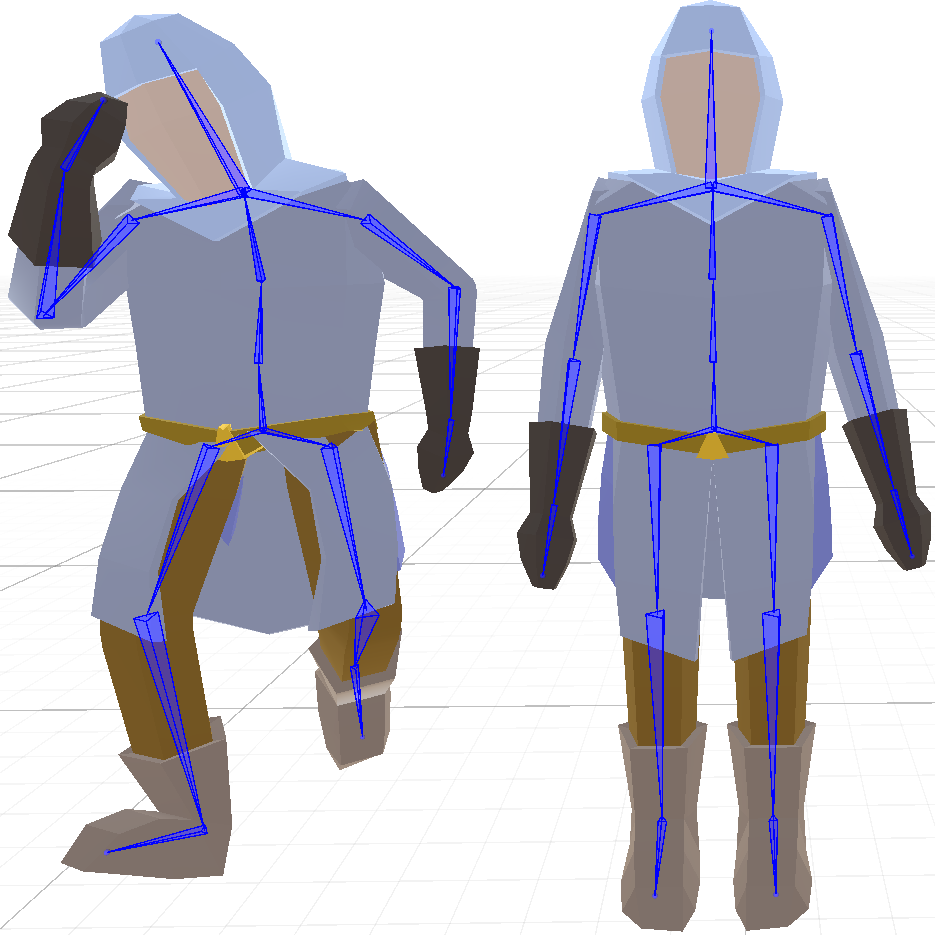
\includegraphics[width=90mm]{../img/boneAnimationDemo.png}
    \caption{Model rytíře s kostmi - póza (nalevo) VS standardní postoj}
    \label{obr03:animationBones}
\end{figure} 
K sofistikovanějšímu pohybu modelem nám tedy stačí v modelovacím programu vytvořit tyto kosti, zahrnout je do exportovaného 3D modelu a v průběhu hry měnit jejich polohy. Unity nám toto umožní přímočaře - po importu modelu do scény v něm kosti najdeme jako obyčejnou hierarchii prázdných herních objektů. Doplňovat je bude druhý podobjekt s komponentou \textit{SkinnedMeshRenderer}, která zajišťuje samotné vykreslení a ví, jak při něm model podle kostí deformovat.

\subsection{Animace}

V typické hře je třeba tímto způsobem vykonávat napříč velkým množstvím modelů velmi složité pohyby, které jsou předpřipravené a ručně vyladěné. Modelovací nástroje jsou typicky vybavené pokročilým editorem pro tvorbu takovýchto animací, které lze následně rovněž exportovat a použít v Unity. V Unity najdeme pokročilý systém pro jejich přehrávání. 

Základem je komponenta \textit{Animator}. Tu jednoduše umístíme na objekt animovatelného 3D modelu, nakonfigurujeme ji, a ta následně nad pohybem kostí přebere plnou kontrolu. Posíláním zpráv a upravováním animačních proměnných jsme schopni vybírat, která animace se má přehrávat, a kontrolovat některé její parametry, přímou kontrolu nad polohami kostí však ztrácíme. 

V mnoha případech takovéto přehrávání předpřipravených animací postačuje, některé vizuální efekty však činí problém - např. nelze otáčet hlavu postavy za pohybujícím se objektem či polohovat samopal v rukou vojáka přesně ve směru kam hráč míří. Pro řešení takovýchto situací je nutné nad částí animace mít přímou kontrolu skrze skript - v Unity nám nadstavbu, která umožňuje tuto tzv. \textit{procedurální animaci}, poskytuje balíček Animation Rigging \cite{AnimationRigging}.


\section{Shrnutí}

Unity je velmi vyspělý engine, který za sebou má desetiletí vývoje a s jeho pomocí bylo vytvořeno mnoho komerčně úspěšných her. Pro svou velmi přívětivou cenovou politiku a možnost kompilovat hry pro širokou škálu platforem od konzolí po mobilní zařízení se stal \textbf{oblíbeným nástrojem začínajících vývojářů a malých týmů}. Uživateli poskytuje mnoho nástrojů a knihoven, od editoru scény po subsystém pro navigaci entit v herním světě. Libovolnou další funkcionalitu lze přidat pomocí skriptů v jazyce C\#. 

Herní scéna je hierarchií objektů - každý z nich je definován svým předkem, jménem, transformační maticí a listem komponent. Komponenty jsou základním stavebním prvkem, kterým dodáváme objektům jejich vlastnosti - např. schopnost mít vizuální reprezentaci, schopnost kolidovat s okolními objekty. Unity poskytuje mnoho předpřipravených komponent, uživatel může definovat vlastní jako skripty dědící z třídy MonoBehavior.

Jednou ze zajímavých skupin komponent jsou ty poskytnuté vestavěným \textbf{fyzikálním sybsystémem}. Jejich prostřednictvím je uživateli poskytnuto rozhraní odpovídající velké podmnožině systému Nvidia PhysX \cite{PhysX}. 

Základem je komponenta Rigidbody - jejím přidáním se z objektu stává fyzikální entita, na kterou lze působit silami. Chceme-li fyzikálnímu objektu umožnit kolidovat s dalšími objekty, přidáme mu jednu nebo více komponent typu Collider. Pro vytváření složitějších vztahů a závislostí mezi jednotlivými fyzikálními tělesy slouží Jointy - s jejich pomocí můžeme vytvořit například dveře otevíratelné v pantech či realisticky se chovající kovový řetěz.

Fyzikální simulace je velmi mocný nástroj, nevytváří však věrný obraz reality. Na mnoha místech narážíme na numerickou stabilitu a také zkrátka na fakt, že hlavní prioritou nikdy nebyla dokonalá přesnost, nýbrž schopnost vyhodnocení v reálném čase.
